%!TEX root = main.tex
\onehalfspacing
In the following experiment the effects of ego depletion on social risk with regard to con-sumer behaviour and behaviour in general will be examined. In order to analyse social risk and consumer behaviour the experiment aims for a decision between products with supposedly high versus low social risk. The second part of the questionnaire includes a scenario in which participants were confronted with criminal cases (judges’ dilemma). This test was included in order to check if ego depletion has an effect on social risk related decision-making in different contexts as well and not only in the context of purchase decisions, thus possibly supporting our results. Participants were provided with information of the respective perpetrator’s criminal record\footnote{All judges’ cases are fictitious} and his/her behaviour in custody. The awareness of responsibility regarding the decision if a ‘delinquent remains in custody’ or ‘will be granted probation’ involves the concept of social risk.
The main components of the empirical research are divided into three subcategories. 
\begin{enumerate}
\item The depletion task (Stroop test)
\item The self-evaluation 
\item The decision-making task (products/judges’ dilemma)
\end{enumerate}
Before the structure of the questionaire will be discussed in detail, the two parts of the question-naire have to be examined. Under the assumption that social risk is a significant factor in the decision-making process, two pre-tests of the survey were implemented. Both parts aim at the aspect of decision-making and social risk. The first and main part focuses on the decision-making process (as part of a purchase decision) under ego depletion, whereas the second part observes the decision-making process in judicial decisions under ego depletion. 
\section{Pre-Test}
The pre-tests were designed in order to define the framework of ‘social risk’. Therefore, we conducted one questionnaire, which dealt with the question of social risk regarding consumer decisions. The other one observed the term of social risk in regard to judicial cases. Both pre-tests will be more closely examined in the two following subsections.
\subsection{Consumer Choice}\label{sec:consumerchoice}
The sample consisted of 34 students (21 male / 13 female) aged between 19 and 32 (m = 25.41; SD = 4.28) enrolled at the University of Hamburg. The main dependent measure for the pre-test was social risk on consumer choice. Participants were presented with a set of products. Each product could be distinguished by one attribute, either colour or design. Partici-pants were randomly assigned to two groups and were shown sets of either five or six products, depending on the group. Each product was presented in five different colours or designs. \par
In the first step, participants were instructed to rank all five versions of the same prod-uct according to social risk. The following definition of social risk was given: (a) the colour or design of which they would most likely expect positive reactions of their social environment (low risk) versus (b) the product of which they would most likely expect adverse reactions of their social environment (high risk). In the second step, participants had to rank all five ver-sions according to personal preference (in the following referred to as ‘liking scale’). The last step aimed for a consumer decision. Participants had to rank the product itself with the help of a Likert scale, with the variables being (a) social risk and (b) design as significant for a purchase decision. An example of the questionnaire is pictured in figure \ref{fig:pretest_sample_shoes}. To emphasize the scale visually in the questionnaire a grey shadowed triangle was put behind the scale.\par
\begin{figure}[h!]
\center
	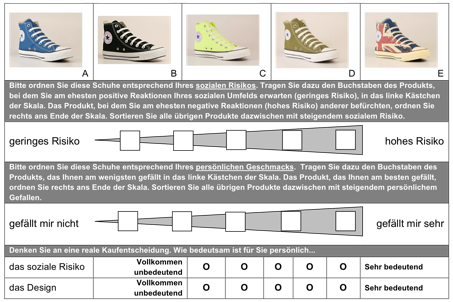
\includegraphics[width=1\textwidth]{images/pretest_sample_shoes.png}
  \caption{Example of questions raised in the pre-test (products) are displayed. The upper task requests to estimate the ‘social risk’ of the product. The following task requests to estimate the ‘liking’ of the product. The lower task re-quests to estimate the personal importance of ‘social risk’ and ‘design’ in a purchase decision.}\label{fig:pretest_sample_shoes}
\end{figure}
Products were chosen to be part of the final questionnaire based on the premise that they pro-vided an approximately equivalent liking and a preferably diverse social risk. Four of the elev-en products complied with our expectations (shoes, sofa, wine, mp3 player and car). \par
Figure \ref{fig:pretest_shoes} displays the five alternatives regarding the product ‘shoes’. The variation ‘black’ with a low ‘social risk’ rating and the variation ‘yellow’ with a high ‘social risk’ rating would indicate the maximum of difference between the variable ‘social risk’. The ‘liking’ rate of these two product variations, however, show also the highest deviation. Therefore, we de-cided to select the product ‘shoe’ with the attribute ‘blue’ (SR = 2.06; liking = 3.50) as the low social risk, and the ‘union jack’ (SR =  4.12; liking = 2.87) as the high social risk alterna-tive. In addition the product choices regarding the variable ‘liking’ corresponded more strongly with each other. \par
% \begin{figure}[h!]
% \center
% 	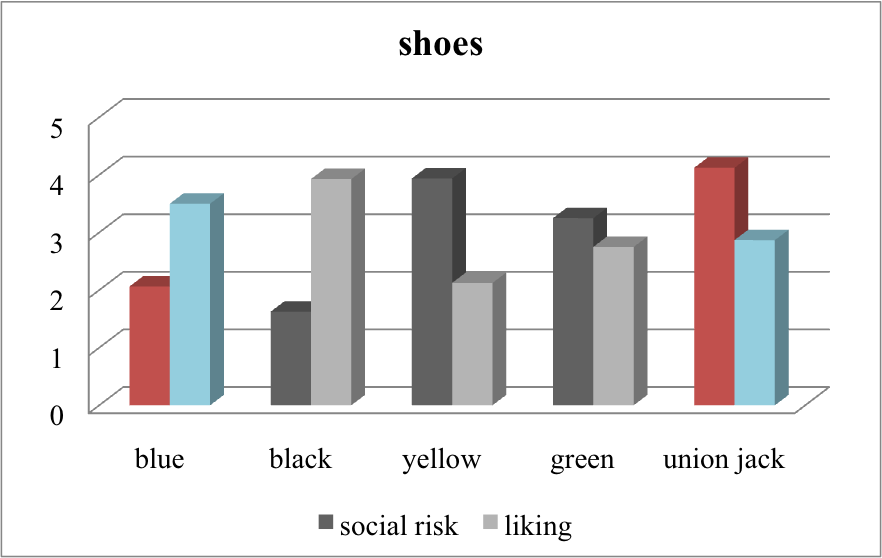
\includegraphics[width=0.9\textwidth]{images/pretest_shoes.png}
%   \caption{The results of the pre-test with regard to the product ‘shoes’ are displayed. The chosen products for the final survey are highlighted in colour (‘social risk’= red and ‘liking’ = blue). The ordinate denotes ‘social risk’ and ‘liking’ on a scale ranging from zero to five. The abscissa denotes the product in five different ‘colour’ variants.}\label{fig:pretest_shoes}
% \end{figure}
Figure \ref{fig:pretest_mp3} displays the options for the product ‘mp3 player’. In this case we decided to select the product ‘mp3 player’ with the attribute ‘yellow’ (SR = 3.88; liking = 2.71) which corresponds more strongly with alternative ‘red’ in regard to the ‘liking’ (SR =  3.29; liking = 2.59). Although, the disparity of social risk would have been higher with the ‘purple’ mp3 player, we decided that the equality of the ‘liking’ as a comparable foundation appears to be more important than finding the highest possible difference in value regarding the item social risk.\par
% \begin{figure}[h!]
% \center
% 	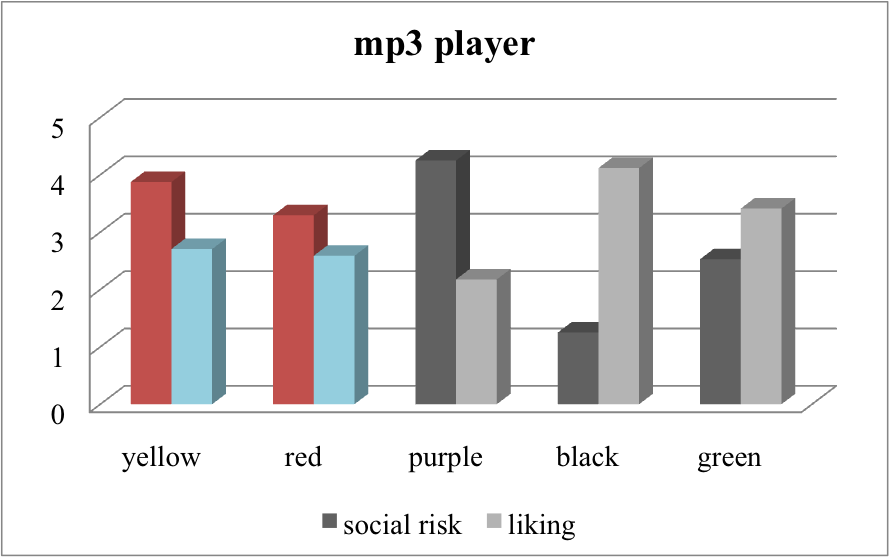
\includegraphics[width=0.9\textwidth]{images/pretest_mp3.png}
%   \caption{The results of the pre-test with regard to the product ‘mp3 player’ are displayed. The chosen products for the final survey are highlighted in colour (‘social risk’= red and ‘liking’ = blue). The ordinate denotes ‘social risk’ and ‘liking’ on a scale ranging from zero to five. The abscissa denotes the product in five different ‘colour’ variants.}\label{fig:pretest_mp3}
% \end{figure}
Figure \ref{fig:pretest_sofa} displays the options for the product ‘sofa’. In this case we decided to select the product ‘sofa’ with the attribute ‘red’ (SR = 3.88; liking = 3.19) which corresponds more strongly with alternative ‘grey’ in regard to the ‘liking’ (SR = 2.69; liking = 3.25). Again, we decided that the equality of the ‘liking’ as a comparable foundation appears to be more im-portant than finding the highest possible difference in value regarding the item social risk. \par
% \begin{figure}[h!]
% \center
% 	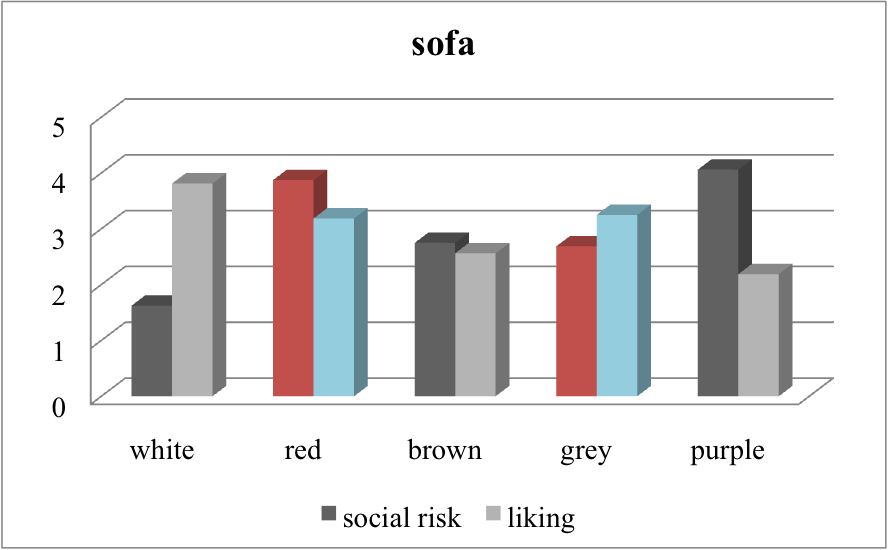
\includegraphics[width=0.9\textwidth]{images/pretest_sofa.png}
%   \caption{The results of the pre-test with regard to the product ‘sofa’ are displayed. The chosen products for the final survey are highlighted in colour (‘social risk’= red and ‘liking’ = blue). The ordinate denotes ‘social risk’ and ‘liking’ on a scale ranging from zero to five. The abscissa denotes the product in five different ‘colour’ variants.}\label{fig:pretest_sofa}
% \end{figure}
Figure \ref{fig:pretest_cars} displays the five alternatives regarding the product ‘car’. This time the distinctive attribute is ‘design’ not ‘colour’. For this purpose we chose five different cars from the same manufacturer and in the same colour. Therefore, we decided to select the product ‘car’ with the attribute ‘limousine’ (SR = 2.12; liking = 2.94) as the low social risk, and the ‘SUV’ (SR =  3.41; liking = 3.29) as the high social risk alternative. In addition the product choices regard-ing the variable ‘liking’ corresponded more strongly with each other than the other possible combinations.\par
% \begin{figure}[h!]
% \center
% 	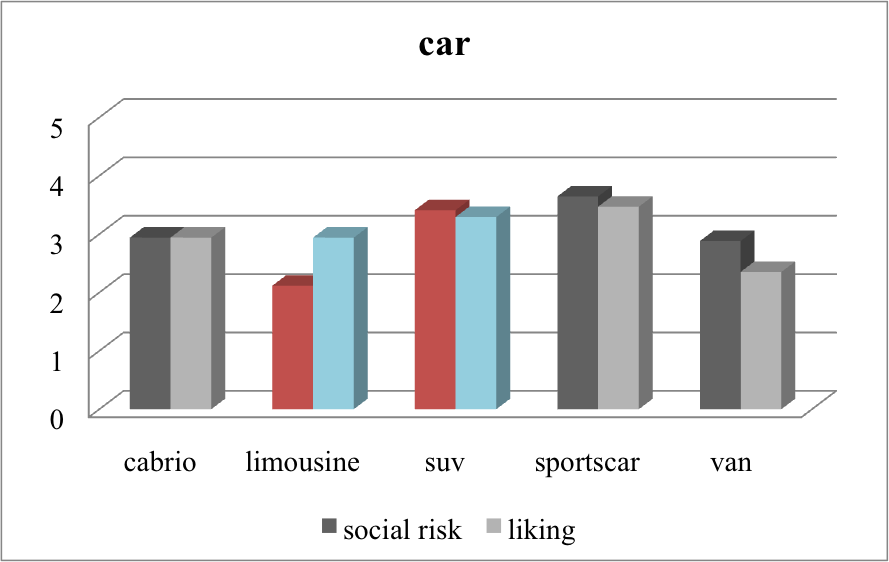
\includegraphics[width=0.9\textwidth]{images/pretest_cars.png}
%   \caption{The results of the pre-test with regard to the product ‘cars’ are displayed. The chosen products for the final survey are highlighted in colour (‘social risk’= red and ‘liking’ = blue). The ordinate denotes ‘social risk’ and ‘liking’ on a scale ranging from zero to five. The abscissa denotes the product in five different ‘design’ variants.}\label{fig:pretest_cars}
% \end{figure}
Figure \ref{fig:pretest_wine} displays the options for the product ‘wine label’. In this case we decided to select the product ‘wine label’ with the attribute ‘white/green’ (SR = 3.36; liking = 3.07) as the high ‘social risk’ item, which also corresponds with the strongest alternative and low ‘social risk’ item ‘green/gold’ regarding the ‘liking’ (SR =  2.50; liking = 3.21). \par
% \begin{figure}[h!]
% \center
% 	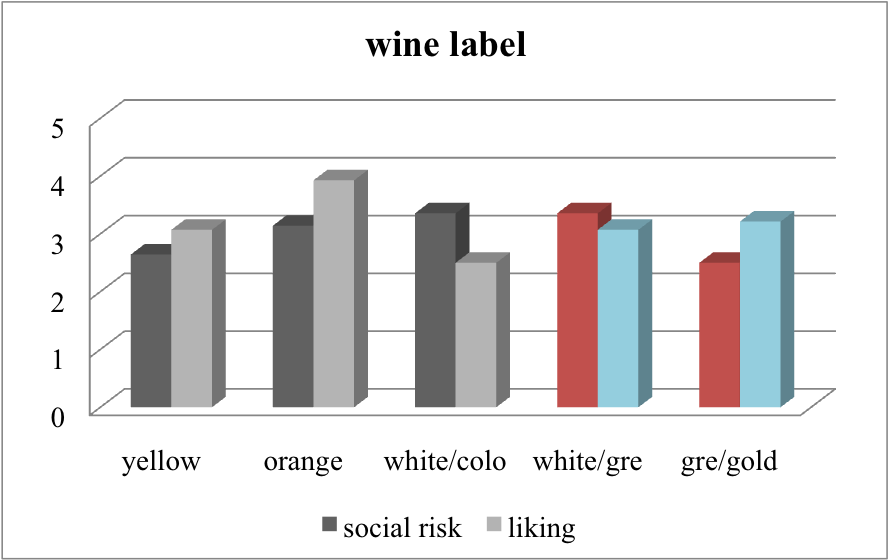
\includegraphics[width=0.9\textwidth]{images/pretest_wine.png}
%   \caption{The results of the pre-test with regard to the product ‘wine label’ are displayed. The chosen products for the final survey are highlighted in colour (‘social risk’= red and ‘liking’ = blue). The ordinate denotes ‘social risk’ and ‘liking’ on a scale ranging from zero to five. The abscissa denotes the product in five different ‘colour’ variants.}\label{fig:pretest_wine}
% \end{figure}

\begin{figure}[h!]
  \begin{center}
    % \showthe\columnwidth % Use this to determine the width of the figure.
    \subfloat[shoes]{\label{fig:pretest_shoes}
		\begin{tikzpicture}[text depth=3pt]
		\tikzstyle{every node}=[style={font=\footnotesize\vphantom{Ag}}]
		\node at (0,0) {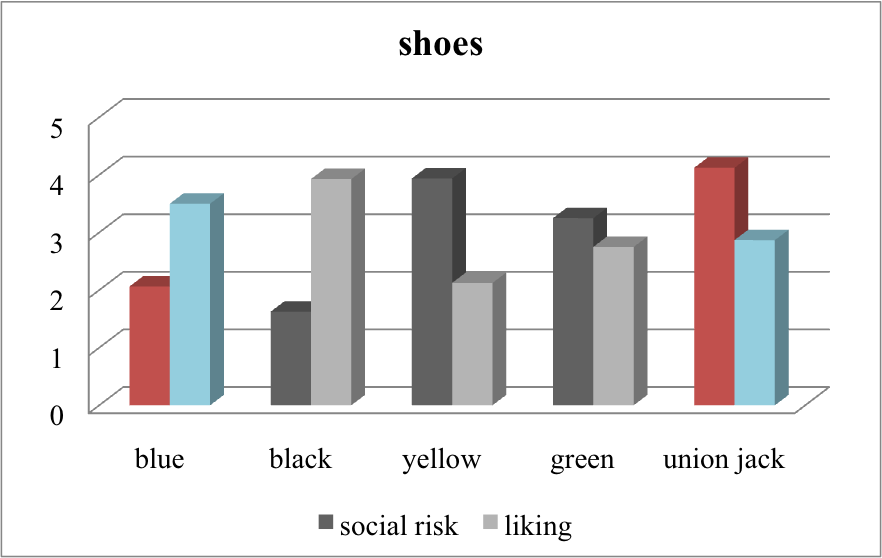
\includegraphics[trim= 1.1cm 2.4cm 3pt 1.6cm,clip=true,width=220pt]{images/pretest_shoes}};
		\draw (-4,-1.5) node(A){0} ++(0,0.55) node(B){1} ++(0,0.55) node(C){2} ++(0,0.55) node(D){3} ++(0,0.55) node(E){4} ++(0,0.55) node(F){5};
		\draw (-2.85,-2) node[](A1){blue} ++(1.36,0) node[](B1){black} ++(1.36,0) node[](C1){yellow} ++(1.36,0) node[](D1){green} ++(1.36,0) node[](E1){union jack};
	% \node [label={[label distance=1cm]30:label}] {Node};	
		  \node[shape=circle split,
		    inner sep= 0pt,
		    label={[yshift=-15pt, xshift=22pt]liking},
		    minimum size = 10pt,
		    line width=0pt,text=white,font=\bfseries,
		    circle split part fill={likingcyan,likinggrey}
		    ] at (-2,-2.7) {};
		  \node[shape=circle split,
		    inner sep= 0pt,
		    label={[yshift=-15pt, xshift=32pt]social risk},
		    minimum size = 10pt,
		    line width=0pt,text=white,font=\bfseries,
		    circle split part fill={riskred,riskdarkgrey}
		    ] at (0,-2.7) {};
		\end{tikzpicture}}
    \subfloat[mp3 player]{\label{fig:pretest_mp3}
		\begin{tikzpicture}[text depth=3pt]
		\tikzstyle{every node}=[style={font=\footnotesize\vphantom{Ag}}]
		\node at (0,0) {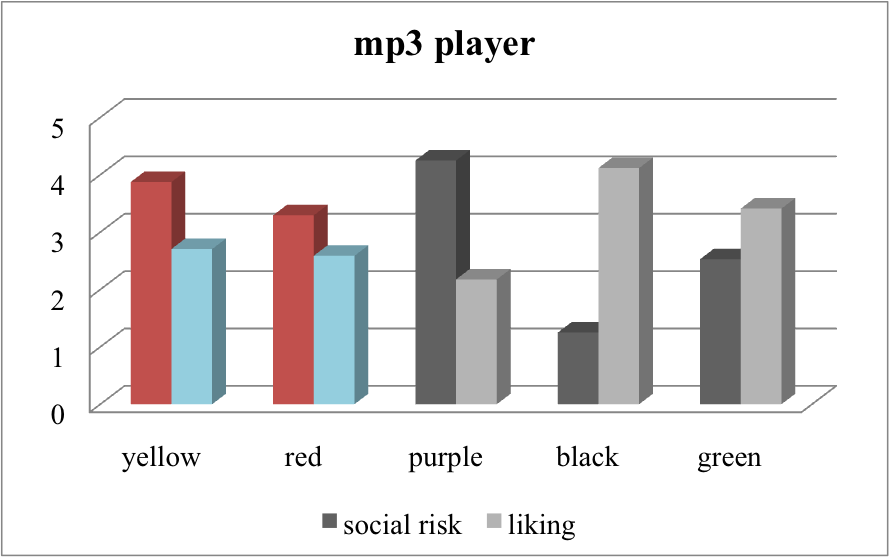
\includegraphics[trim= 1.1cm 2.4cm 3pt 1.6cm,clip=true,width=220pt]{images/pretest_mp3}};
		\draw (-4,-1.5) node(A){0} ++(0,0.55) node(B){1} ++(0,0.55) node(C){2} ++(0,0.55) node(D){3} ++(0,0.55) node(E){4} ++(0,0.55) node(F){5};
		\draw (-2.85,-2) node[](A1){yellow} ++(1.36,0) node[](B1){red} ++(1.36,0) node[](C1){purple} ++(1.36,0) node[](D1){black} ++(1.36,0) node[](E1){green};
	   %  \clip (0,0) circle (8pt);
    % \begin{scope}
    %     \fill[likinggrey] (-3,-3) rectangle (0,3);
    %     \fill[likingcyan] (-0.001,3) rectangle (3,-3);
    % \end{scope}
		  \node[shape=circle split,
		    inner sep= 0pt,
		    label={[yshift=-15pt, xshift=22pt]liking},
		    minimum size = 10pt,
		    line width=0pt,text=white,font=\bfseries,
		    circle split part fill={likingcyan,likinggrey}
		    ] at (-2,-2.7) {};
		  \node[shape=circle split,
		    inner sep= 0pt,
		    label={[yshift=-15pt, xshift=32pt]social risk},
		    minimum size = 10pt,
		    line width=0pt,text=white,font=\bfseries,
		    circle split part fill={riskred,riskdarkgrey}
		    ] at (0,-2.7) {};
		% \draw \fill[color=red!20 (0,0) circle (1ex);
		\end{tikzpicture}
		}
    \caption{The results of the pre-tests with regard to the product ‘shoes’ and ‘mp3 player’ are displayed. The chosen products for the final questionnaire are highlighted in colour (‘social risk’= red and ‘liking’ = blue). The ordinate denotes ‘social risk’ and ‘liking’ on a scale ranging from zero to five. The abscissa denotes the product in five different ‘colour’ variants.}\label{fig:pretests_shoes_mp3}
  \end{center}
\end{figure}

\begin{figure}[h!]
  \begin{center}
    % \showthe\columnwidth % Use this to determine the width of the figure.
    \subfloat[sofa]{\label{fig:pretest_sofa}
		\begin{tikzpicture}[text depth=3pt]
		\tikzstyle{every node}=[style={font=\footnotesize\vphantom{Ag}}]
		\node at (0,0) {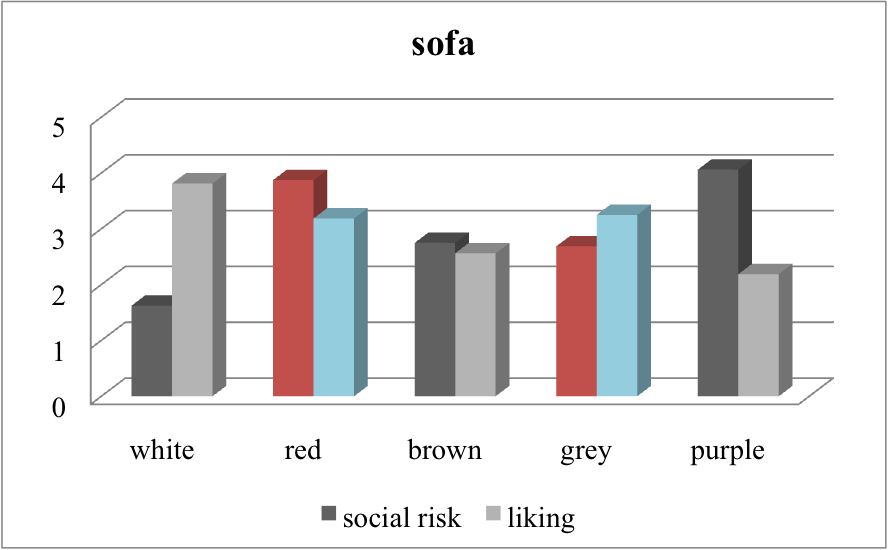
\includegraphics[trim= 1.1cm 2.4cm 3pt 1.6cm,clip=true,width=220pt]{images/pretest_sofa}};
		\draw (-4,-1.5) node(A){0} ++(0,0.55) node(B){1} ++(0,0.55) node(C){2} ++(0,0.55) node(D){3} ++(0,0.55) node(E){4} ++(0,0.55) node(F){5};
		\draw (-2.85,-2) node[](A1){white} ++(1.36,0) node[](B1){red} ++(1.36,0) node[](C1){brown} ++(1.36,0) node[](D1){grey} ++(1.36,0) node[](E1){purple};
	% \node [label={[label distance=1cm]30:label}] {Node};	
		  \node[shape=circle split,
		    inner sep= 0pt,
		    label={[yshift=-15pt, xshift=22pt]liking},
		    minimum size = 10pt,
		    line width=0pt,text=white,font=\bfseries,
		    circle split part fill={likingcyan,likinggrey}
		    ] at (-2,-2.7) {};
		  \node[shape=circle split,
		    inner sep= 0pt,
		    label={[yshift=-15pt, xshift=32pt]social risk},
		    minimum size = 10pt,
		    line width=0pt,text=white,font=\bfseries,
		    circle split part fill={riskred,riskdarkgrey}
		    ] at (0,-2.7) {};
		\end{tikzpicture}}
    \subfloat[cars]{\label{fig:pretest_cars}
		\begin{tikzpicture}[text depth=3pt]
		\tikzstyle{every node}=[style={font=\footnotesize\vphantom{Ag}}]
		\node at (0,0) {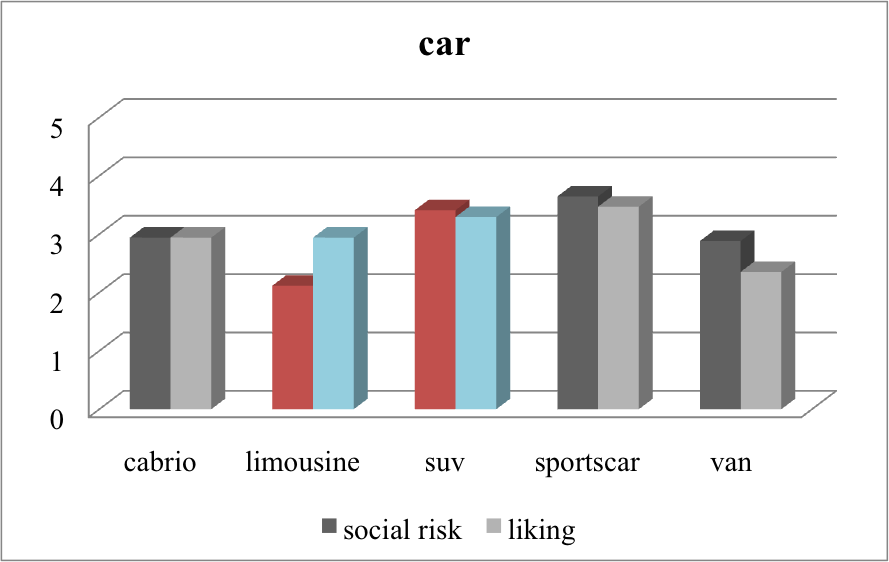
\includegraphics[trim= 1.1cm 2.4cm 3pt 1.6cm,clip=true,width=220pt]{images/pretest_cars}};
		\draw (-4,-1.5) node(A){0} ++(0,0.55) node(B){1} ++(0,0.55) node(C){2} ++(0,0.55) node(D){3} ++(0,0.55) node(E){4} ++(0,0.55) node(F){5};
		\draw (-2.85,-2) node[](A1){cabrio} ++(1.36,0) node[](B1){limousine} ++(1.36,0) node[](C1){SUV} ++(1.36,0) node[](D1){sportscar} ++(1.36,0) node[](E1){Van};
	   %  \clip (0,0) circle (8pt);
    % \begin{scope}
    %     \fill[likinggrey] (-3,-3) rectangle (0,3);
    %     \fill[likingcyan] (-0.001,3) rectangle (3,-3);
    % \end{scope}
		  \node[shape=circle split,
		    inner sep= 0pt,
		    label={[yshift=-15pt, xshift=22pt]liking},
		    minimum size = 10pt,
		    line width=0pt,text=white,font=\bfseries,
		    circle split part fill={likingcyan,likinggrey}
		    ] at (-2,-2.7) {};
		  \node[shape=circle split,
		    inner sep= 0pt,
		    label={[yshift=-15pt, xshift=32pt]social risk},
		    minimum size = 10pt,
		    line width=0pt,text=white,font=\bfseries,
		    circle split part fill={riskred,riskdarkgrey}
		    ] at (0,-2.7) {};
		% \draw \fill[color=red!20 (0,0) circle (1ex);
		\end{tikzpicture}
		}
    \caption{The results of the pre-tests with regard to the product ‘sofa’ and ‘cars’ are displayed. The chosen products for the final questionnaire are highlighted in colour (‘social risk’= red and ‘liking’ = blue). The ordinate denotes ‘social risk’ and ‘liking’ on a scale ranging from zero to five. (a) The abscissa denotes the product in five different ‘colour’ variants. (b) The abscissa denotes the product in five different ‘design’ variants.}\label{fig:pretests_sofa_car}
  \end{center}
\end{figure}

\begin{figure}[h!]
  \begin{center}
    % \showthe\columnwidth % Use this to determine the width of the figure.
    \subfloat[wine label]{\label{fig:pretest_wine}
		\begin{tikzpicture}[text depth=3pt]
		\tikzstyle{every node}=[style={font=\footnotesize\vphantom{Ag}}]
		\node at (0,0) {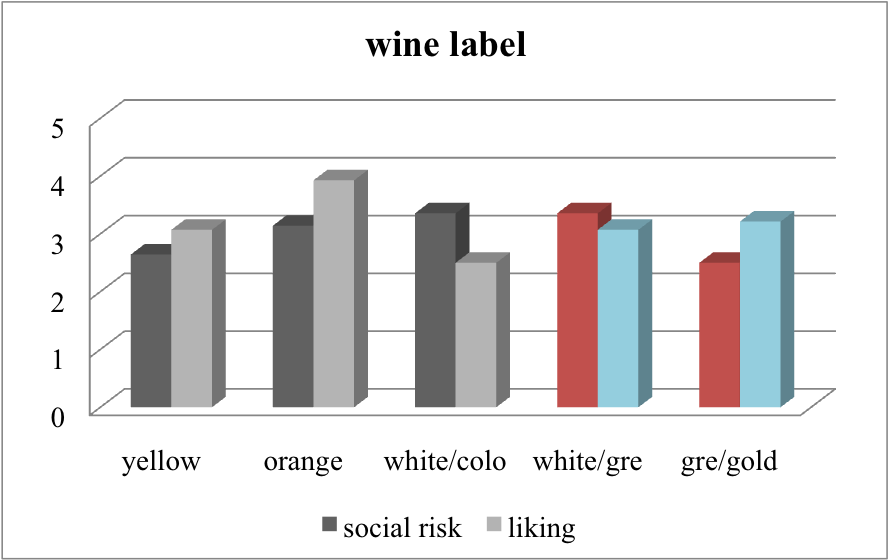
\includegraphics[trim= 1.1cm 2.4cm 3pt 1.6cm,clip=true,width=220pt]{images/pretest_wine}};
		\draw (-4,-1.5) node(A){0} ++(0,0.55) node(B){1} ++(0,0.55) node(C){2} ++(0,0.55) node(D){3} ++(0,0.55) node(E){4} ++(0,0.55) node(F){5};
		\draw (-2.85,-2) node[](A1){yellow} ++(1.36,0) node[](B1){orange} ++(1.36,0) node[yshift=-6pt,align=center](C1){white/\\clrd} ++(1.36,0) node[yshift=-6pt,align=center](D1){white/\\green} ++(1.36,0) node[yshift=-6pt,align=center](E1){green/\\gold};
	% \node [label={[label distance=1cm]30:label}] {Node};	
		  \node[shape=circle split,
		    inner sep= 0pt,
		    label={[yshift=-15pt, xshift=22pt]liking},
		    minimum size = 10pt,
		    line width=0pt,text=white,font=\bfseries,
		    circle split part fill={likingcyan,likinggrey}
		    ] at (-2,-2.7) {};
		  \node[shape=circle split,
		    inner sep= 0pt,
		    label={[yshift=-15pt, xshift=32pt]social risk},
		    minimum size = 10pt,
		    line width=0pt,text=white,font=\bfseries,
		    circle split part fill={riskred,riskdarkgrey}
		    ] at (0,-2.7) {};
		\end{tikzpicture}
		}
    \caption{The results of the pre-test with regard to the product ‘wine label’ are displayed. The chosen products for the final questionnaire are highlighted in colour (‘social risk’= red and ‘liking’ = blue). The ordinate denotes ‘social risk’ and ‘liking’ on a scale ranging from zero to five. The abscissa denotes the product in five different ‘colour’ variants.}\label{fig:pretests_wine}
  \end{center}
\end{figure}


\subsection{Judges’ dilemma}
The pre-test sample consisted of nine students enrolled at the University of Hamburg. They were given eight scenarios. Each scenario described a case of a delinquent. The case provided information about the crime and the delinquent’s behaviour in prison. Even though the cases differed from each other, they were all based on certain fundamental conditions. All delinquents were (a) between the age of 20 and 30 and were (b) sentenced to between eight and twelve years and (c) had served at least half of their custodial sentence. The scenarios were e.g. designed as follows: “Michael Truman (aged 29) kidnapped a politician's son (aged 12). He demanded 4 million USD. After the transaction Michael Truman was caught and the boy was freed. However, the money has never been found. He was sentenced to 12 years. During his time in prison Michael Truman did not have a negative record. Michael Truman is filing for probation after being in prison for 6 years.“\par
With this information at hand participants had to decide which perpetrator had to remain in custody or would be granted probation. In this pre-test, social risk was defined as responsibility (social consequences). Participants were instructed to keep in mind that resocialization is an important objective, so is keeping in custody a possible repeater.\par
Figure \ref{fig:pretest_judges} shows the distribution of decisions made by the participants. The y-axis displays the experiments which were exposed to the subjects, and the x-axis shows the ratio of decisions (Probation / no Probation). More participants tended in experiment 2 and 7 towards ‘no probation’, whereas more subjects with respect to experiment 4 and 5 leaned towards ‘probation’. Four of the eight scenarios complied with our expectations and three experiments were accepted due to high rate of difficulty for the subjects to decide (Exp. 1, Exp. 6 and Exp. 8). To examine the questionnaire regarding the pre-test (judges’ dilemma) more closely please see Appendix.

\begin{figure}[h!]
\center
	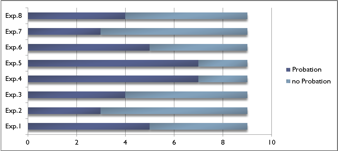
\includegraphics[width=0.9\textwidth]{images/pretest_judges.png}
  \caption{The results of the pre-test in regard to the cases’ of the ‘judges’ dilemma’ are dis-played. The decisions of the participants are highlighted in colour (‘probation’= violet and ‘no probation’ = blue). The ordinate denotes the experiment. The abscissa denotes the share of decisions in favour or against.}\label{fig:pretest_judges}
\end{figure}

\section{Depletion Task and Decision Making}
\subsection{Stroop Test}
In the former \citep{muraven1998self,baumeister2002yielding} and the current \citep{unger2011ego,pocheptsova2009deciding} debate on ego depletion several approaches to deplete experimental groups were implemented. Most of them were based on depletion under self-regulation. The Stroop test \citep{stroop1935studies} seemed to be the most adaptive instrument to deplete participants under the construct of an online questionnaire. The depletion task with the Stroop test (experimental condition) was grouped into three sets each containing 60 questions. The participants were presented with three sets each containing 60 words denoting colours. They were instructed to name the colour not the written word by clicking on the appropriately labelled button. If the colour of the written word was blue, they were told to name the word, not the denoting colour. Furthermore, they were instructed to answer quickly and do not pause during the sets. After each set participants were informed how many answers were given correctly. For the control group a similar test, without the depletion task, was designed. The control group had to name the colour by clicking on the appropriately labelled button. However, the denoting colour was always dark grey. It was assumed that the control group were therefore able to concentrate on the word itself without cognitively suppressing the written word or the colour (see Figure 10). 

\begin{figure}[h!]
  \begin{center}
    % \showthe\columnwidth % Use this to determine the width of the figure.
    \subfloat[control group]{\label{fig:os_green}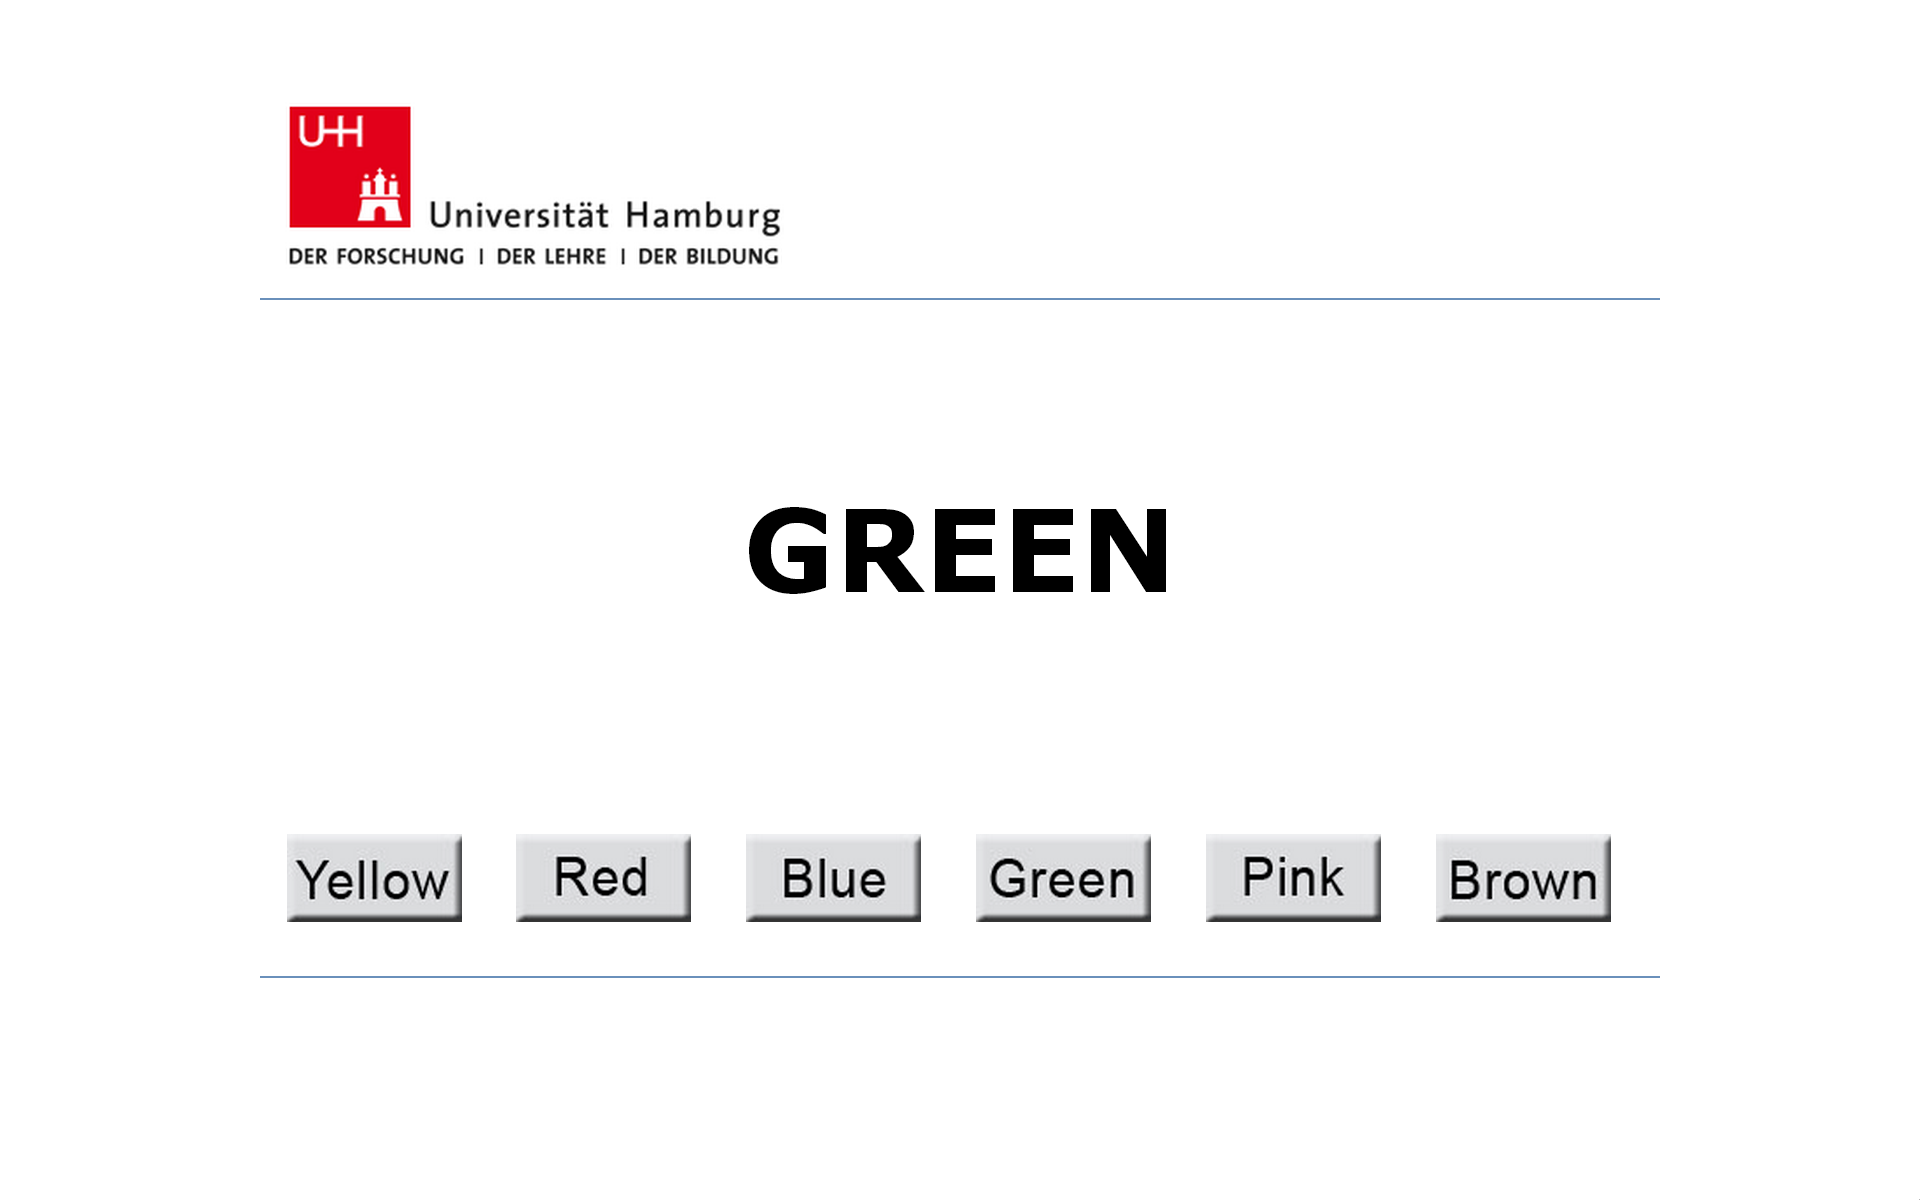
\includegraphics[trim= 0cm 0cm 0pt 0cm,clip=true,width=220pt]{images/os_green}}
    \subfloat[wine label]{\label{fig:os_pink}
\includegraphics[trim= 0cm 0cm 0pt 0cm,clip=true,width=220pt]{images/os_pink}}
    \caption{Example of Stroop test. (a) Left side (control group = nondepletion). (b) Right side (experimental group = depletion)}\label{fig:green_vs_pink}
  \end{center}
\end{figure}

\subsection{Product Choice}
The products used in the final questionnaire were preselected according to results of the pre-test (compare pre-test Chapter 3.1.1). Two versions of each product were chosen which showed both similar ‘liking’ ratings and a preferably diverse rating of ‘social risk’. \par
Figure \ref{fig:decision_process} Example of a decision process in regard to product choice in the pre-test \par
In the first step, a comparable foundation had to be established. Colour was the only dis-tinctive feature of the products. Two versions of each product (those which had received a similar  ‘liking’ rate in the pre-test) were chosen to be integrated into the final questionnaire. In order to provide a clear option of choice between high and low risk for the participants, a preferably high difference of social risk was the determining factor in the second step, in which products had to fulfil the following conditions in order to be included in the question-naire (compare Chapter \ref{sec:consumerchoice}).\par

\begin{figure}[h!]
\center
	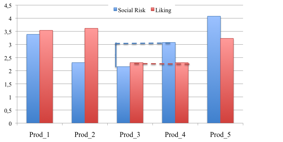
\includegraphics[width=0.9\textwidth]{images/pretest_sample.png}
  \caption{Example of a decision process in regard to product choice in the pre-test}\label{fig:decision_process}
\end{figure}

\subsection{Judges’ Choice}\label{sec:judgeschoice}
Danziger, Levav and Avnaim-Presso \citep{danziger2011extraneous} observed over a time period of ten months 1,112 judicial sentences. They assumed that judges who have to decide upon complicated cases simplify their decisions over the day and will therefore be more tempted to accept the status quo (prisoner remains in custody) instead of the alternative (grant the prisoner’s request of probation).\par
As Figure \ref{fig:decisions_danziger} shows, the ruling in favour of the accused had its peaks in the morning and right after the breaks. They came to the conclusion that “\emph{[\ldots] the likelihood of a favourable ruling is greater at the very beginning of the work day or after a food break than later in the sequence of cases [\ldots]}” \citep[p.~6890]{danziger2011extraneous}. It became clear that for perpetrators it is a non-judicial advantage to have a trial in the morning and not in the afternoon. Danziger, Levav and Avnaim-Presso assumed that the second and third peak after the breaks had to do with the intake of nutrition. Or how they put it “\emph{[\ldots] justice is “what the judge ate for break-fast [\ldots]}”“ \cite[p.~6889]{danziger2011extraneous}. \todo{double quotation marks?}\par
To adapt this theory, fictitious cases were designed and pre-tested (compare Chapter \ref{sec:consumerchoice}). Three of the eight cases were chosen. The participants labelled all chosen cases as ‘difficult to answer’ and ‘an ambiguous decision’. Taking the inconclusive cases into the questionnaire, it was assumed that the depleted subjects would lean towards the decision ‘remain in custody’ (risk aversion) rather than ‘will be granted probation’ (non risk aversion). Consequently, a different decision pattern, showing a less ‘conservative’ approach, was expected in the non-depleted control group.\par

\begin{figure}[h!]
\center
	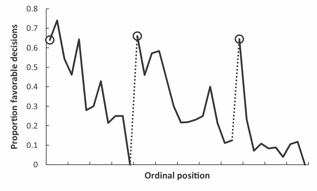
\includegraphics[width=0.9\textwidth]{images/JD_decisions_danziger.png}
  \caption{“Proportion of rulings in favor of the prisoners by ordinal position. Circled points indicate the first decision in each of the three decision sessions; tick marks on x axis denote every third case; dotted line denotes food break. Be-cause unequal session lengths resulted in a low number of cases for some of the later ordinal positions, the graph is based on the first 95\% of the data from each session.“ \citep{danziger2011extraneous}}\label{fig:decisions_danziger}
\end{figure}

\section{Depletion Measure and Self-Evaluation}
The last part of the questionnaire was designed to measure the level of depletion among participants of the experimental group and the control group. To approach this issue from two different angles it was decided to create the first element of the last part as a depletion meas-ure task and the second element as a self-evaluation test.
\subsection{Measuring Self-Control and Consumer Behaviour}
Accurate measurement of self-control and consumer behaviour is a critical issue. With the combination of three different Likert scales it was intended to picture a pattern within both groups (depletion vs. non-depletion). To assess participants’ self-evaluation concerning spend-ing behaviour and general self-control three Likert scales were applied. The General Self-Control scale (SCS) “\emph{[\ldots] is designed to capture differences in general self-control as expressed through control over thoughts, impulse control, emotional control, habit breaking, and performance regulation}” \citep{tangney2004high}. As discussed in Chapter \ref{chap:effectsofegodepletion}, it is probably more difficult to deplete people who generally possess a high level of self-control through self-regulation. Therefore, it seemed appropriate to distinguish between participants showing high and low levels of self-control. Five of 36 possible statements on a five-point Likert scale (with agreement ranging from ‘not at all’ to ‘very much’) were chosen for this purpose.\par
The Exploratory Tendencies in Consumer Behavior (CBS) \citep{raju1980optimum} were used to distinguish between purchasers who (a) tend to buy what they know and purchasers who (b) are open to buy new products. “\emph{The 39 items were classified into these categories based on the wording of the items and inter-item correlations [\ldots]}“ \citep{raju1980optimum}. Raju categorized participants of his study into the following seven categories.\par

\begin{enumerate}[label=\emph{\alph*}.]
\item [”\stepcounter{enumi}\emph{\alph{enumi}}.]\emph{Repetitive behaviour proneness: the tendency to stick with the same response over time. }
\item \emph{Innovativeness: eagerness to buy or know about new products/services. }
\item \emph{Risk taking: a preference for taking risks or being adventurous. }
\item \emph{Exploration through shopping: a preference for shopping and investigating brands. }
\item \emph{Interpersonal communication: communicating with friends about purchases. }
\item \emph{Brand switching: switching brands primarily for change or variety. }
\item \emph{Information seeking: interest in knowing about various products and brands mainly out of curiosity.}” \citep{raju1980optimum}
\end{enumerate}
Four of 36 possible statements on a seven-point Likert scale (with agreement ranging from ‘not at all’ to ‘very much’) were chosen for this purpose.\par
The last scale used to assess participants’ self-evaluation was the Consumer Spending Self-Control (SSC). It was conceptualized „\emph{[\ldots] as an individual difference, distinct from general self-control, develop a parsimonious measure to assess it, and demonstrate important related consequences and behaviors. Furthermore, we provide direct evidence that it is a differential focus on future outcomes that drives the distinct responses of high- versus low-CSSC consumers to the provision of outcome elaboration prompts}” \citep{haws2012consumer}. Four of 10 possible statements on a five-point Likert scale (with agreement ranging from ‘not at all’ to ‘very much’) were chosen for this purpose.\par

\subsection{Depletion Measure}
In order to compare the level of depletion (experimental group vs. control group) four questions from the cognitive reflection test were integrated into the questionnaire. These ques-tions were originally designed to assess a specific cognitive ability \citep{frederick2005cognitive}. In this case, however, it was assumed that the experimental group would provide less correct re-sponses than the control group. For the use of our questionnaire we chose four questions, con-structed in a way that the subjects perceive the task as easy and fast to answer. This task aims exactly at the first impulse answer, which supposedly is in general the wrong one.  Figure \ref{fig:os_depletion_measure}displays an example of the depletion task. In this case the supposedly impulse reaction would be the answer ‘24 days’. The correct answer, however, is ‘47 days’.  \par

\begin{figure}[h!]
\center
	
\includegraphics[width=0.9\textwidth]{images/os_depletion_measure.png}
  \caption{Example of the depletion measure task (own design)}\label{fig:os_depletion_measure}
\end{figure}

\subsection{Depletion Self-Evaluation}\label{sec:depletionself-evaluation}
The final part of the questionnaire contained two additional Likert scales. In the cognitive reflection test (depletion measure) we aimed for a neutral measurement of depletion. The self-evaluation was implemented to assess if the perceived degree of difficulty (five-point scale from ‘not at all exhausted’ to ‘very exhausted’) and the perceived degree of exhaustion (five-point scale from ‘very easy’ to ‘very difficult’) complied each other. Moreover we wanted to examine the relation between the difficulty and exhaustion and the results by the objective depletion measure. The results could provide us with information about the perceived depletion and if the result drew the same picture as the depletion task itself. 

\section{Online Questionnaire}
Summing up, the questionnaire consists of:
\begin{enumerate}
\item An introduction: The participants are informed of the following questionnaire without informing them what the questionnaire is aiming at. 
\item A socio-demographic questionnaire: Participants are asked to indicate their age, gen-der, nationality and level of education.
\item A self-evaluation questionnaire: Participants inform about their consumer behaviour and their perceptive self-regulation behaviour.
\item A depletion task: Based on the Stroop theory (depletion trough self-regulation exhaustion), also known as Stroop test.  
\item A product choice questionnaire: Participants have to decide which product they prefer. With every product choice, subjects are given additional information regarding the purchase.
\item A social-consequences questionnaire: Participants have to decide towards which decision they lean. With each judges’ case, subjects are given additional information re-garding the perpetrator.
\item A depletion-measuring task: Participants are asked to answer questions, in order to as-sess their ability to answer them correctly after being depleted (or non-depleted).
\item A second self-evaluation questionnaire: Participants inform about their perceived level of exhaustion and their perceived level of difficulty of the test.
\end{enumerate}

This chapter has clarified how social risk is defined in the framework of this experiment and how ego depletion is generated in the experimental group.  In addition, it has been dis-cussed at length how products and the judicial cases were selected for the decision-making part of the questionnaire. In the next chapter we will briefly sketch the method of the online sequence and subsequently present the results. Considering the findings (see Chapter 4.2)\todo{replace with ref}, we will try to examine how ego depletion affects decision-making and social risk. \par
The following chapter shows a description of the related test material, the pre-tests, the sample population and the test procedure, followed by a presentation of the overall results of this study.\par

